%%%%%%%%%%%%%%%%%%%%%%%%%%%%%%%%%%%%%%%%%%%%%%%%%%%%%%%%%%%%%%%%%%%%%%%%%%%%%%%
%                                                                             %
% Anwendungsbeispiel für das Beamer-Template TU Chemnitz                      %
% (c) Mario Haustein (mario.haustein@hrz.tu-chemnitz.de), 2013-2014           %
%                                                                             %
%%%%%%%%%%%%%%%%%%%%%%%%%%%%%%%%%%%%%%%%%%%%%%%%%%%%%%%%%%%%%%%%%%%%%%%%%%%%%%%

\usepackage[utf8]{inputenc}
\usepackage[ngerman]{babel}



% TUC-Templates laden.
\usetheme{tuc2014}
\mode<article>{\usepackage{beamerarticletuc2014}}


%
% Weitere Anpassungen nach Bedarf.
%

%% Navigationsleiste deaktivieren.
\setbeamertemplate{navigation symbols}{}

%% Mathematische Sätze nummerieren.
%\setbeamertemplate{theorems}[numbered]

%% Titelzeile fett und in Standardfarbe formatieren.
%\setbeamercolor{frametitle}{parent=normal text}
%\setbeamerfont{frametitle}{series=\bfseries}



% Metadaten
\title[Modellierung und Integration von Sensorknoten in Omnet++]{Modellierung und Integration von Sensorknoten in einer Simulationsumgebung}
\subtitle{Bachelorarbeit}
\author{Thomas Rückert}
\date{\today}
\institute[TUC]{TU Chemnitz}
\titlegraphic{
\includegraphics[height=0.2\textheight]{tuc2014/logo/tuc_green}}
\tucurl{http://www.tu-chemnitz.de/urz/}



\begin{document}
\tucthreeheadlines
\frame{\titlepage}
\note{Anmerkungen}

\frame{
\frametitle{kurze Einführung}
\begin{itemize}
\item Sensoren 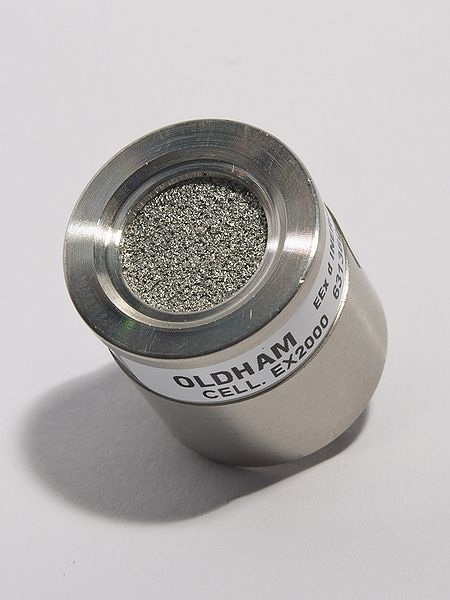
\includegraphics[height=0.3\textheight]{450px-Gas-Sensor}
\item Netzwerke aus Sensorknoten - WSN \\
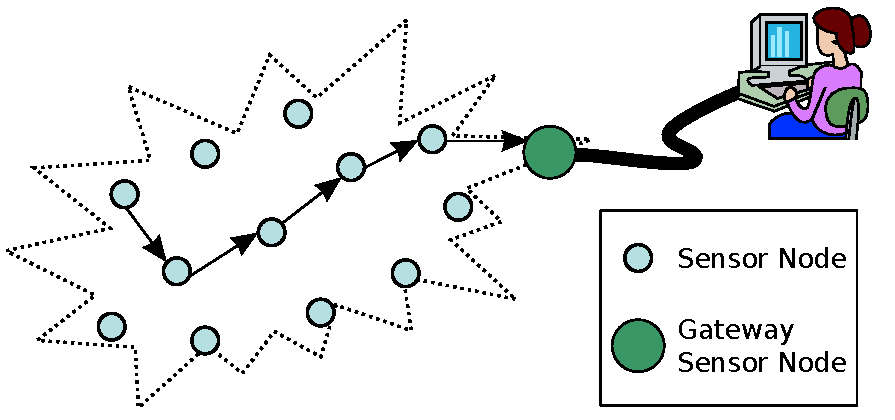
\includegraphics[height=0.3\textheight]{WSN}
\end{itemize}
}

\note{
\begin{itemize}
\item lateinisch sentire, dt. fühlen oder empfinden
\item WSN - wireless sensor network
\end{itemize}
}

\tuctwoheadlines
\frame{\frametitle{Gliederung}\tableofcontents}
\note{\begin{itemize}
\item Weitere Anmerkungen \dots
\item \dots\ in Stichpunkten \dots
\item \dots\ formuliert.
\end{itemize}}

%
% Inhalt
%

\section{Einleitung}

\frame<beamer| trans>{
\Huge\begin{center}\scalebox{2}{\texttt{Einleitung}}\end{center}
}

\note {

}

\subsection{Aufgabe}
\frame<beamer| trans>{
\frametitle{Thema}
\begin{center}
"Modellierung und Integration von Sensorknoten in einer Simulationsumgebung"
\end{center}
}

\note{
\begin{itemize}
\item Grundlagen von
\begin{itemize}
\item Simulationsumgebung OMNET++ mit MiXiM
\item Verwaltung und Bereitstellung von Umgebungs-/Umweltparametern
\item Auswertung von Simulationsdaten / Visualisierung
\end{itemize}
\item Modellierung mehrerer unterschiedlicher Sensorknoten (Hosts) 
\begin{itemize}
\item Integration von Sensorik zur Erfassung der Umgebungsparameter
\item Betrachtung des Energiehaushaltes bei Sensornutzung
\item Modellierung und Test (Beispielanwendung auf Sensorknoten)
\end{itemize}
\item Erstellung einer Simulationsumgebung 
\begin{itemize}
\item Nutzung von vielen und unterschiedlichen Sensorknoten
\item Modellierung, Datenvisualisierung und Test
\end{itemize}
\end{itemize}
}

\section{Vorbetrachtungen}

\subsection{Simulation vs. Emulation und Prototyping}
\frame<beamer| trans>{
\large Simulation vs. Emulation und Prototyping\\
\normalsize
\begin{itemize}
\item \textbf{Simulationen}
\item Emulation
\item Prototyping
\end{itemize}
}

\note {

}

\subsection{Sensoren}
\frame<beamer| trans>{
}

\note {

}

\section{Umsetzung}

\subsection{Omnet++}
\frame<beamer| trans>{
}

\note {

}

\subsection{bisherige Anwendung}
\frame<beamer| trans>{

}

\note {

}

\subsection{Beispiel}

\frame<beamer| trans>{
}

\note {

}

\section{}
\frame<beamer| trans>{\Huge\begin{center}\scalebox{2}{\texttt{ENDE}}\end{center}}

\note {

}

\begin{onlyenv}<beamer| trans>
\appendix
\newcounter{finalframe}
\setcounter{finalframe}{\value{framenumber}}


%
% "Spare-Slides" hier einsetzen.
%

\frame<beamer| trans>{
ich bin bonus
}

\note {

}

\setcounter{framenumber}{\value{finalframe}}
\end{onlyenv}
\end{document}
